\chapter{Metodologia}
% ---
% ---
Neste segmento, serão delineadas informações relacionadas à elaboração da aplicação proposta neste projeto. Discutiremos a Estruturação do desenvolvimento, a Análise de requisitos, abrangendo tanto os funcionais quanto os não funcionais.

Para a realização deste trabalho, em termos de sua natureza, foi adotada a metodologia de pesquisa aplicada. Conforme \begin{citacao}
	\cite{fleury2016pesquisa}
	a pesquisa aplicada concentra-se em torno dos problemas presentes nas atividades das instituições, organizações, grupos ou atores sociais. Ela está empenhada na elaboração de 
    diagnósticos, identificação de problemas e busca de soluções
\end{citacao} 

\section{Estruturação do desenvolvimento}
A forma como foi organizado o desenvolvimento do presente trabalho foi dividio em etapas, sendo elas:
\begin{itemize}
	\item Análise de Requisitos
	\item Criação da estrutura para armazenamento de dados
	\item Desenvolvimento da aplicação Web
\end{itemize}

Conforme demonstrado na \autoref{fig:grafico-etapas-desenvolvimento}:

\begin{figure}[htb]
    \caption{\label{fig:grafico-etapas-desenvolvimento}Etapas de Desenvolvimento}
    \begin{center}
        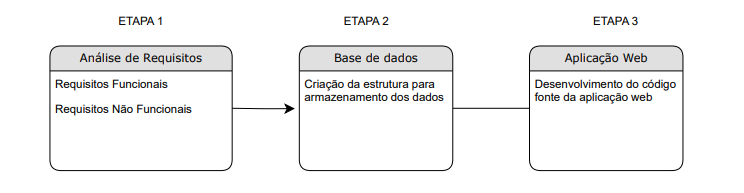
\includegraphics[scale=0.9]{imagens/estagios-de-desenvolvimento.png}
    \end{center}
\end{figure}


\section{Análise de Requisitos}
Os requisitos inerentes a aplicação web AutoForm foram identificados por meio de entrevistas conduzidas com um membro do setor de Tecnologia da Brigada Militar, SD. Tiago Costa. Durante essas entrevistas, foram formuladas perguntas pertinentes ao procedimento de geração do AEL.

A coleta de dados foi complementada por meio da análise de documentos, da portaria 136 Anexo D. Esta nota conceitua todas as fases envolvidas na execução dos Testes de Avaliação Física da Brigada Militar do Rio Grande do Sul. Nesse contexto, foram examinadas as deficiências identificadas na Brigada, a fim de informar o desenvolvimento tanto do aplicativo quanto do sistema. Ademais, foi realizada uma avaliação para determinar as funcionalidades essenciais para o pleno funcionamento de ambos os sistemas.

\subsection{Requisitos Funcionais}
Os requisitos funcionais são aqueles que descrevem as funcionalidades que o sistema deve possuir. Para o desenvolvimento da aplicação AutoForm, foram identificados os seguintes requisitos funcionais:

\subsection{Requisitos Não Funcionais}
Os requisitos não funcionais são aqueles que descrevem as características que o sistema deve possuir. Para o desenvolvimento da aplicação AutoForm, foram identificados os seguintes requisitos não funcionais:

% % ---
% \section{Tabelas}
% % ---

% \index{tabelas}A \autoref{tab-nivinv} é um exemplo de tabela construída em
% \LaTeX.

% \begin{table}[htb]
% \ABNTEXfontereduzida
% \caption[Níveis de investigação]{Níveis de investigação.}
% \label{tab-nivinv}
% \begin{tabular}{p{2.6cm}|p{6.0cm}|p{2.25cm}|p{3.40cm}}
%   %\hline
%    \textbf{Nível de Investigação} & \textbf{Insumos}  & \textbf{Sistemas de Investigação}  & \textbf{Produtos}  \\
%     \hline
%     Meta-nível & Filosofia\index{filosofia} da Ciência  & Epistemologia &
%     Paradigma  \\
%     \hline
%     Nível do objeto & Paradigmas do metanível e evidências do nível inferior &
%     Ciência  & Teorias e modelos \\
%     \hline
%     Nível inferior & Modelos e métodos do nível do objeto e problemas do nível inferior & Prática & Solução de problemas  \\
%    % \hline
% \end{tabular}
% \legend{Fonte: \citeonline{van86}}
% \end{table}

% Já a \autoref{tabela-ibge} apresenta uma tabela criada conforme o padrão do
% \citeonline{ibge1993} requerido pelas normas da ABNT para documentos técnicos e
% acadêmicos.

% \begin{table}[htb]
% \IBGEtab{%
%   \caption{Um Exemplo de tabela alinhada que pode ser longa
%   ou curta, conforme padrão IBGE.}%
%   \label{tabela-ibge}
% }{%
%   \begin{tabular}{ccc}
%   \toprule
%    Nome & Nascimento & Documento \\
%   \midrule \midrule
%    Maria da Silva & 11/11/1111 & 111.111.111-11 \\
%   \midrule 
%    João Souza & 11/11/2111 & 211.111.111-11 \\
%   \midrule 
%    Laura Vicuña & 05/04/1891 & 3111.111.111-11 \\
%   \bottomrule
% \end{tabular}%
% }{%
%   \fonte{Produzido pelos autores.}%
%   \nota{Esta é uma nota, que diz que os dados são baseados na
%   regressão linear.}%
%   \nota[Anotações]{Uma anotação adicional, que pode ser seguida de várias
%   outras.}%
%   }
% \end{table}
% ---


